\chapter{Theoretische Grundlagen}
%-------------------------------------------------------------------------------------------------

% - Hier werden die relevanten Theorien und Modelle beschrieben, die für das Verständnis der Arbeit notwendig sind.
% - Falls du auf bestehende wissenschaftliche Literatur zurückgreifst, solltest du diese hier zusammenfassen und die wichtigsten Konzepte erläutern.

%-------------------------------------------------------------------------------------------------
\section{Glosar und Akronyme}
%-------------------------------------------------------------------------------------------------
%-------------------------------------------------------------------------------------------------

\gls{latex} ist ein leistungsfähiges Werkzeug zum Setzen von wissenschaftlichen Arbeiten.
In dieser Arbeit wird \gls{latex} verwendet, um das Dokument zu erstellen. Außerdem kam \gls{chatgpt} zum Einsatz, um Texte zu verbessern. Die \acrshort{hsrm} bietet eine Vielzahl an technischen Studiengängen. 
Die \acrshort{hsrm} ist bekannt für ihre technischen Studiengänge. Die \acrfull{hsrm} bietet viele Möglichkeiten für Forschung und Lehre.



%-------------------------------------------------------------------------------------------------
\section{Zitieren}
%-------------------------------------------------------------------------------------------------
%-------------------------------------------------------------------------------------------------

Hier schreiben Sie den Text für Ihr Thema hinein.

sfas \cite{ChatGPTl} \cite{Richard.2020} \cite{Fushimi.Mehrzyklone} \cite{Schlegel.MedPhy.2018}

In wissenschaftlichen Arbeiten ist es wichtig, die verwendeten Quellen korrekt zu zitieren. Hier sind einige Beispiele, wie man nach dem IEEE-Stil zitiert:

\begin{itemize}
    \item \textbf{Einfaches Zitat}: Ein einfaches Zitat mit einer Nummer in eckigen Klammern: \cite{ChatGPTl}. Dies ist der übliche Stil nach IEEE.
    \item \textbf{Mehrere Quellen}: Es ist auch möglich, mehrere Quellen gleichzeitig zu zitieren: \cite{Richard.2020, Fushimi.Mehrzyklone}. Die Zitate werden automatisch nummeriert.
\end{itemize}

Zusätzlich wird im IEEE-Stil oft eine nummerierte Liste im Literaturverzeichnis verwendet, um alle Quellen aufzulisten. Achten Sie darauf, die Nummerierung konsistent zu halten.

Weitere Hinweise:
- Im IEEE-Stil werden die Autoren in der Reihenfolge des Erscheinens zitiert.
- Stellen Sie sicher, dass alle verwendeten Quellen auch im Literaturverzeichnis aufgelistet sind.


%-------------------------------------------------------------------------------------------------
\section{Abbildungen}
%-------------------------------------------------------------------------------------------------
%-------------------------------------------------------------------------------------------------

\begin{figure}[H]
    \centering
    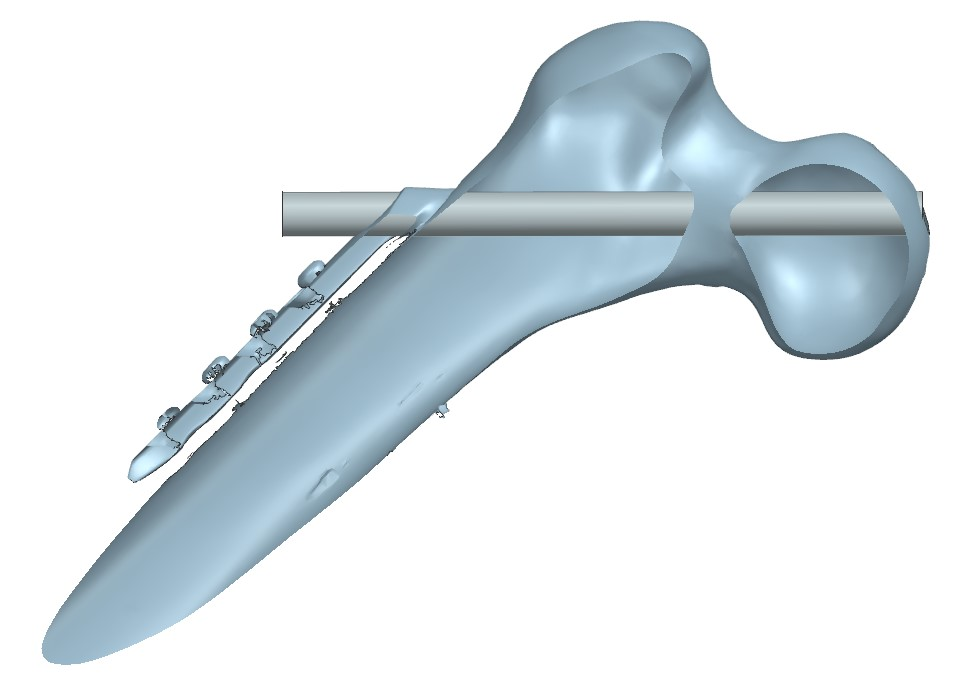
\includegraphics[width=0.6\textwidth]{abb1/bohrschablone_Seitenansicht.jpg} % Anpassung der Breite des Bildes
    \caption{Bohrschablone \cite{ChatGPTl}}
    \label{bild groß}
\end{figure}



\begin{figure}[H]
    \centering
    \begin{minipage}{0.4\textwidth}
        \centering
        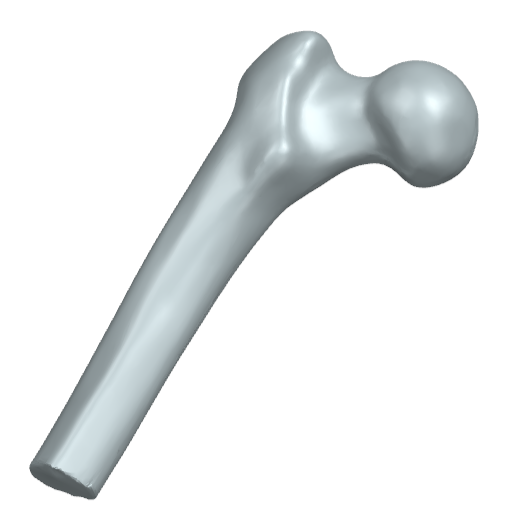
\includegraphics[width=\textwidth]{abb1/Femur_oben_GOM.png}
        \caption{einstein Bodybuilding}
        \label{fig:bildMitText}
    \end{minipage}
    \hfill
    \begin{minipage}{0.55\textwidth}
        \textbf{Beschreibung:}\\
        Dies ist ein Beispiel für einen Textabschnitt neben einem Bild. Hier können Sie eine ausführliche Beschreibung des Bildes oder andere relevante Informationen hinzufügen.
    \end{minipage}
\end{figure}



\begin{figure}[H]
    \centering
    \begin{minipage}[b]{0.3\textwidth}
        \centering
        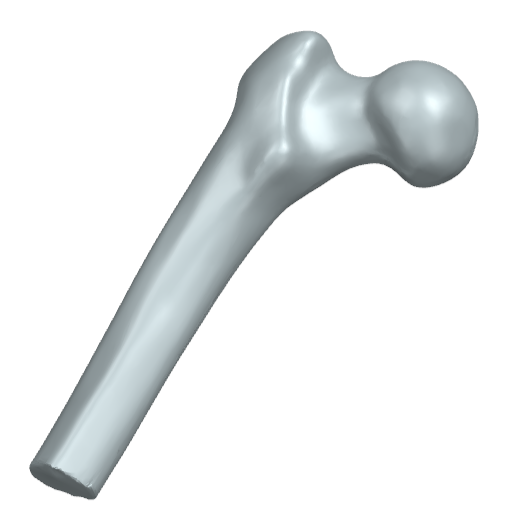
\includegraphics[width=\textwidth]{abb1/Femur_oben_GOM.png}
        \caption{Bild 1}
    \end{minipage}
    \hfill
    \begin{minipage}[b]{0.3\textwidth}
        \centering
        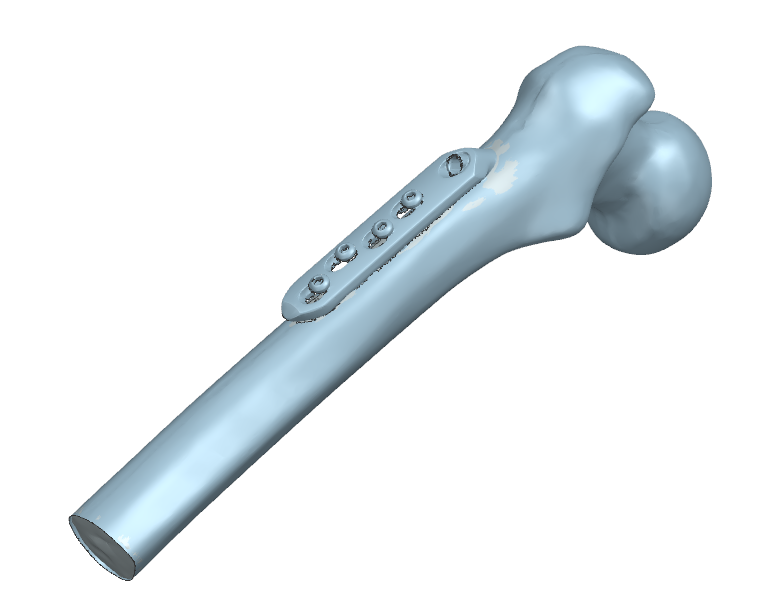
\includegraphics[width=\textwidth]{abb1/Impl_2_3D_Scan.png}
        \caption{Bild 2}
    \end{minipage}
    \hfill
    \begin{minipage}[b]{0.3\textwidth}
        \centering
        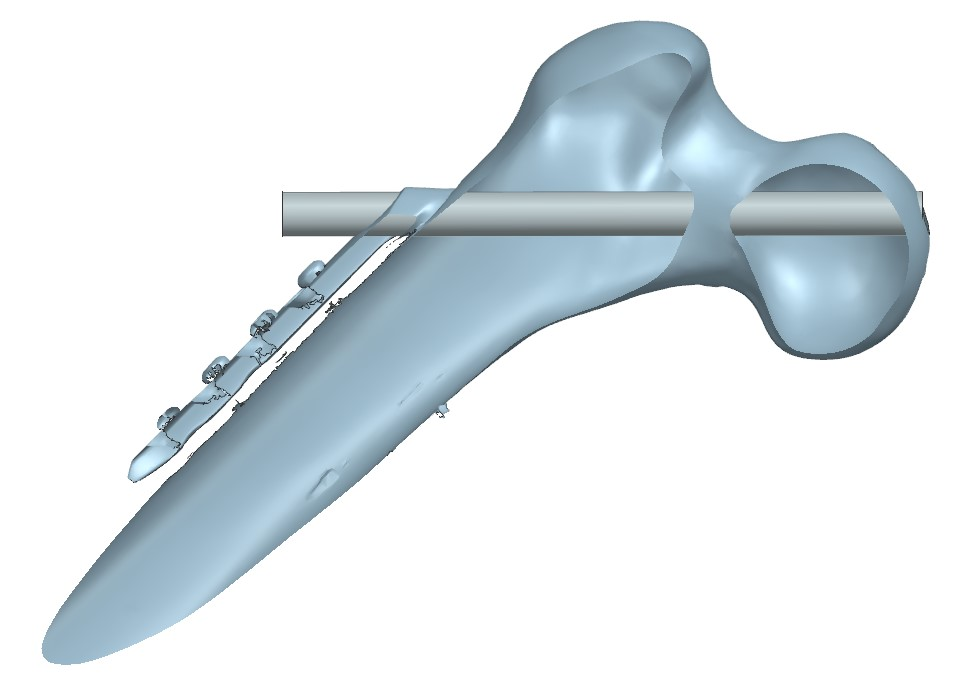
\includegraphics[width=\textwidth]{abb1/bohrschablone_Seitenansicht.jpg}
        \caption{Bild 3}
    \end{minipage}
\end{figure}



%-------------------------------------------------------------------------------------------------
\section{Tabellen}
%-------------------------------------------------------------------------------------------------
%-------------------------------------------------------------------------------------------------

\textbf{TABELLEN HABEN ÜBERSCHRIFTEN UND BILDER HABEN UNTERSCHRIFTEN!!!}

% Tabelle mit Vergleich zwischen Katzen und Raben
\begin{table}[H]
    \centering
    \caption{Vergleich zwischen Katzen und Raben}
    \begin{tabular}{|c|c|c|}
        \hline
        \textbf{Eigenschaft} & \textbf{Katzen} & \textbf{Raben} \\
        \hline
        Lebensdauer & 12-18 Jahre & 10-15 Jahre \\
        \hline
        Gewicht & 4-5 kg & 0.7-1.4 kg \\
        \hline
        Nahrung & Fleischfresser & Allesfresser \\
        \hline
        Lebensraum & Haushalte, Wildnis & Wälder, Städte \\
        \hline
        Intelligenz & Hoch & Sehr hoch \\
        \hline
        Soziales Verhalten & Einzelgänger & Gesellig \\
        \hline
    \end{tabular}
    \label{tab:katzen_raben}
\end{table}


\begin{table}[H]
    \centering
    \caption{Bilder in Tabellen}
    \begin{tabular}{c c c}
        \hline
        \textbf{Abbildung 1} & \textbf{Noch ein weiteres Bild} \\
        \hline
            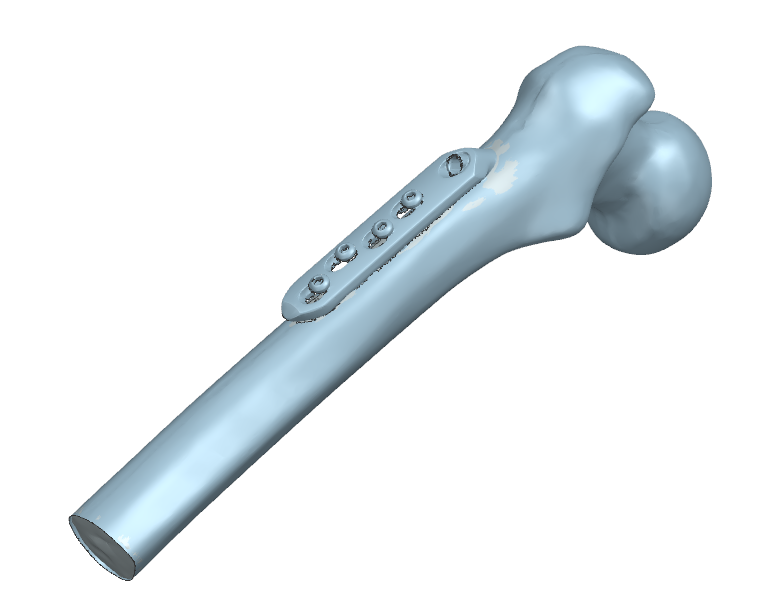
\includegraphics[width=0.2\linewidth]{abb1/Impl_2_3D_Scan.png} & 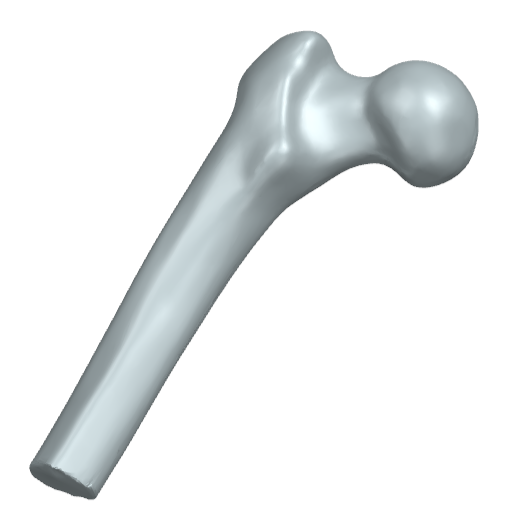
\includegraphics[width=0.2\linewidth]{abb1/Femur_oben_GOM.png} \\ 
        \hline
    \end{tabular}
    \label{BilderTab}
\end{table}


% Tabelle ohne Rahmen
\begin{table}[H]
    \centering
    \caption{Vergleich zwischen Katzen und Raben}
    \begin{tabular}{ c c c }
        \textbf{Eigenschaft} & \textbf{Katzen} & \textbf{Raben} \\
        Lebensdauer & 12-18 Jahre & 10-15 Jahre \\
        Gewicht & 4-5 kg & 0.7-1.4 kg \\
        Nahrung & Fleischfresser & Allesfresser \\
        Lebensraum & Haushalte, Wildnis & Wälder, Städte \\
        Intelligenz & Hoch & Sehr hoch \\
        Soziales Verhalten & Einzelgänger & Gesellig \\
    \end{tabular}
    \label{ohneRahmenTab}
\end{table}


% Tabelle mit nur einem Feld, das ein Bild enthält
\begin{table}[H]
    \centering
    \caption{Tabelle mit nur einem Feld, das ein Bild enthält}
    \begin{tabular}{c}
        \includegraphics[width=0.8\textwidth]{abb1/Gegenüberstellungsmatrix.png} % Pfad zum Bild anpassen
    \end{tabular}
    \label{tab:einBild}
\end{table}


%-------------------------------------------------------------------------------------------------
\section{Mathematisches}
%-------------------------------------------------------------------------------------------------

Hier schreiben Sie den Text für Ihr Thema hinein.

% Einfache Formel im Text
Die berühmte Einstein-Gleichung ist $E = mc^2$.

% Abgesetzte Formel ohne Nummer
\[
E = mc^2 
\]

% Abgesetzte Formel mit Nummer
\begin{equation}
E = mc^2
\label{einstein.eq}
\end{equation}

Gleichung \ref{einstein.eq} ist Einsteins Gleichung.

% Mehrzeilige Formel (Millikan-Versuch)
\begin{align}
q &= ne \\
F &= qE \\
ma &= qE \\
a &= \frac{qE}{m}
\end{align}

% Formel mit Summen und Integralen
\begin{equation}
\int_0^\infty e^{-x^2} \, dx = \frac{\sqrt{\pi}}{2}
\end{equation}

\[
i\hbar \frac{\partial}{\partial t} \Psi(\mathbf{r}, t) = \hat{H} \Psi(\mathbf{r}, t)
\]

% Formel mit Brüchen
\begin{equation}
f(x) = \frac{a}{b} + \frac{c}{d}
\label{eq2}
\end{equation}

% Formel mit griechischen Buchstaben und Exponenten
\begin{equation}
\alpha^2 + \beta^2 = \gamma^2
\label{eq1}
\end{equation}

% Erweiterte Mathematische Beispiele
\begin{equation}
\nabla \times \mathbf{E} = -\frac{\partial \mathbf{B}}{\partial t}
\label{maxwell1}
\end{equation}

\begin{equation}
\oint_\mathcal{C} \mathbf{B} \cdot d\mathbf{l} = \mu_0 I + \mu_0 \epsilon_0 \frac{d\Phi_E}{dt}
\label{maxwell2}
\end{equation}

Hier kann man auch auf Gleichungen verweisen! Gleichungen \ref{maxwell1} und \ref{maxwell2} sind Teil der Maxwell-Gleichungen.

%-------------------------------------------------------------------------------------------------
\section{Code Beispiele}
%-------------------------------------------------------------------------------------------------

\subsection{Python Code}
\begin{minted}[linenos, fontsize=\small]{python}
def fibonacci(n):
    """Berechnet die Fibonacci-Zahlen bis n."""
    a, b = 0, 1
    while a < n:
        print(a, end=' ')
        a, b = b, a + b
    print()
    
fibonacci(1000)
\end{minted}

\subsection{C++ Code}
\begin{minted}[linenos, fontsize=\small]{c++}
#include <iostream>

void fibonacci(int n) {
    int a = 0, b = 1;
    while (a < n) {
        std::cout << a << " ";
        int temp = a;
        a = b;
        b = temp + b;
    }
    std::cout << std::endl;
}

int main() {
    fibonacci(1000);
    return 0;
}
\end{minted}

%-------------------------------------------------------------------------------------------------
\section{Schaltkreise}
%-------------------------------------------------------------------------------------------------

Für Schaltkreise verwenden Sie das \texttt{circuitikz}-Paket:

\begin{figure}[H]
    \centering
    \begin{circuitikz}
        \draw (0,0) to[battery, l=9V] (0,2) to[resistor, l=R] (2,2) to[bulb, l=Glühbirne] (2,0) -- (0,0);
    \end{circuitikz}
    \caption{Ein einfacher Stromkreis mit Batterie, Widerstand und Glühbirne}
    \label{fig:stromkreis}
\end{figure}

%-------------------------------------------------------------------------------------------------
\section{Vektorgrafiken}
%-------------------------------------------------------------------------------------------------

Für Vektorgrafiken verwenden Sie das \texttt{tikz}-Paket:

\begin{figure}[H]
    \centering
    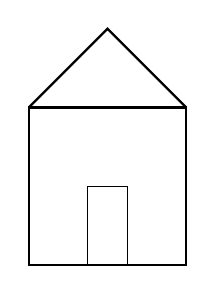
\begin{tikzpicture}
        % Erstellen eines einfachen Hauses
        \draw[thick] (0,0) rectangle (2,2); % Quadrat
        \draw[thick] (0,2) -- (1,3) -- (2,2); % Dach
        \draw (0.75,0) rectangle (1.25,1); % Tür
    \end{tikzpicture}
    \caption{Eine einfache Vektorgrafik: Haus}
    \label{fig:vektorgrafik}
\end{figure}



%-------------------------------------------------------------------------------------------------
\section{Aufzählungen und Listen}
%-------------------------------------------------------------------------------------------------

\subsection{Aufzählungen}
\begin{itemize}
  \item Punkt eins
  \item Punkt zwei
  \item Punkt drei
\end{itemize}

\subsection{Nummerierte Listen}
\begin{enumerate}
  \item Erster Punkt
  \item Zweiter Punkt
  \item Dritter Punkt
\end{enumerate}

\subsection{Verschachtelte Listen}
\begin{itemize}
  \item Erster Punkt
  \begin{itemize}
    \item Unterpunkt eins
    \item Unterpunkt zwei
  \end{itemize}
  \item Zweiter Punkt
\end{itemize}



